%%%%%%%%%%%%%%%%%%%%%%%%%%%%%%%%%%%%%%%%%
% Arsclassica Article
% LaTeX Template
% Version 1.1 (10/6/14)
%
% This template has been downloaded from:
% http://www.LaTeXTemplates.com
%
% Original author:
% Lorenzo Pantieri (http://www.lorenzopantieri.net) with extensive modifications by:
% Vel (vel@latextemplates.com)
%
% License:
% CC BY-NC-SA 3.0 (http://creativecommons.org/licenses/by-nc-sa/3.0/)
%
%%%%%%%%%%%%%%%%%%%%%%%%%%%%%%%%%%%%%%%%%

%----------------------------------------------------------------------------------------
%	PACKAGES AND OTHER DOCUMENT CONFIGURATIONS
%----------------------------------------------------------------------------------------

\documentclass[
10pt, % Main document font size
a4paper, % Paper type, use 'letterpaper' for US Letter paper
oneside, % One page layout (no page indentation)
%twoside, % Two page layout (page indentation for binding and different headers)
headinclude,footinclude, % Extra spacing for the header and footer
BCOR5mm, % Binding correction
]{scrartcl}

%%%%%%%%%%%%%%%%%%%%%%%%%%%%%%%%%%%%%%%%%
% Arsclassica Article
% Structure Specification File
%
% This file has been downloaded from:
% http://www.LaTeXTemplates.com
%
% Original author:
% Lorenzo Pantieri (http://www.lorenzopantieri.net) with extensive modifications by:
% Vel (vel@latextemplates.com)
%
% License:
% CC BY-NC-SA 3.0 (http://creativecommons.org/licenses/by-nc-sa/3.0/)
%
%%%%%%%%%%%%%%%%%%%%%%%%%%%%%%%%%%%%%%%%%

%----------------------------------------------------------------------------------------
%	REQUIRED PACKAGES
%----------------------------------------------------------------------------------------

\usepackage[
nochapters, % Turn off chapters since this is an article        
beramono, % Use the Bera Mono font for monospaced text (\texttt)
eulermath,% Use the Euler font for mathematics
pdfspacing, % Makes use of pdftex’ letter spacing capabilities via the microtype package
dottedtoc % Dotted lines leading to the page numbers in the table of contents
]{classicthesis} % The layout is based on the Classic Thesis style

\usepackage{graphicx}
\usepackage[T1]{fontenc}
\usepackage{textcomp}

\usepackage[utf8x]{inputenc}

\usepackage{gnuplot-lua-tikz}
\usepackage{color}

\usepackage{arsclassica} % Modifies the Classic Thesis package

\usepackage[T1]{fontenc} % Use 8-bit encoding that has 256 glyphs
\usepackage{subfig}
\usepackage{graphicx} % Required for including images
\graphicspath{{Figures/}} % Set the default folder for images

\usepackage{enumitem} % Required for manipulating the whitespace between and within lists

\usepackage{lipsum} % Used for inserting dummy 'Lorem ipsum' text into the template


\usepackage{amsmath,amssymb,amsthm} % For including math equations, theorems, symbols, etc

\usepackage{varioref} % More descriptive referencing

%----------------------------------------------------------------------------------------
%	THEOREM STYLES
%---------------------------------------------------------------------------------------

\theoremstyle{definition} % Define theorem styles here based on the definition style (used for definitions and examples)
\newtheorem{definition}{Definition}

\theoremstyle{plain} % Define theorem styles here based on the plain style (used for theorems, lemmas, propositions)
\newtheorem{theorem}{Theorem}

\theoremstyle{remark} % Define theorem styles here based on the remark style (used for remarks and notes)

%----------------------------------------------------------------------------------------
%	HYPERLINKS
%---------------------------------------------------------------------------------------

\hypersetup{
%draft, % Uncomment to remove all links (useful for printing in black and white)
colorlinks=true, breaklinks=true, bookmarks=true,bookmarksnumbered,
urlcolor=webbrown, linkcolor=RoyalBlue, citecolor=webgreen, % Link colors
pdftitle={}, % PDF title
pdfauthor={\textcopyright}, % PDF Author
pdfsubject={}, % PDF Subject
pdfkeywords={}, % PDF Keywords
pdfcreator={pdfLaTeX}, % PDF Creator
pdfproducer={LaTeX with hyperref and ClassicThesis} % PDF producer
}
 % Include the structure.tex file which specified the document structure and layout

\hyphenation{Fortran hy-phen-ation} % Specify custom hyphenation points in words with dashes where you would like hyphenation to occur, or alternatively, don't put any dashes in a word to stop hyphenation altogether

%----------------------------------------------------------------------------------------
%	TITLE AND AUTHOR(S)
%----------------------------------------------------------------------------------------

\title{\normalfont{Conception d'un outil d'analyse et analyse de la trace d'un réseau en C}} % The article title

\author{\spacedlowsmallcaps{Thibaut EHLINGER}} % The article author(s) - author affiliations need to be specified in the AUTHOR AFFILIATIONS block

\date{Vendredi 27 novembre 2015} % An optional date to appear under the author(s)

%----------------------------------------------------------------------------------------

\begin{document}

%----------------------------------------------------------------------------------------
%	HEADERS
%----------------------------------------------------------------------------------------

\renewcommand{\sectionmark}[1]{\markright{\spacedlowsmallcaps{#1}}} % The header for all pages (oneside) or for even pages (twoside)
%\renewcommand{\subsectionmark}[1]{\markright{\thesubsection~#1}} % Uncomment when using the twoside option - this modifies the header on odd pages
\lehead{\mbox{\llap{\small\thepage\kern1em\color{halfgray} \vline}\color{halfgray}\hspace{0.5em}\rightmark\hfil}} % The header style

\pagestyle{scrheadings} % Enable the headers specified in this block

%----------------------------------------------------------------------------------------
%	TABLE OF CONTENTS & LISTS OF FIGURES AND TABLES
%----------------------------------------------------------------------------------------

\maketitle % Print the title/author/date block


%----------------------------------------------------------------------------------------
%	ABSTRACT
%----------------------------------------------------------------------------------------

\section*{Abstract} % This section will not appear in the table of contents due to the star (\section*)
Ce rapport présente la conception en C d'un utilitaire permettant l'analyse d'un fichier trace d'un réseau fonctionnant pour un certain format de fichier indépendemment de sa taille.

Il y figure aussi quelques pistes concernant les résultats trouvés lors de l'analyse d'un fichier de trafique spécifique fourni par notre encadrant. 

\makeatletter
\newcommand*{\centerfloat}{%
  \parindent \z@
  \leftskip \z@ \@plus 1fil \@minus \textwidth
  \rightskip\leftskip
  \parfillskip \z@skip}
\makeatother
\begin{figure}
	\centerfloat
   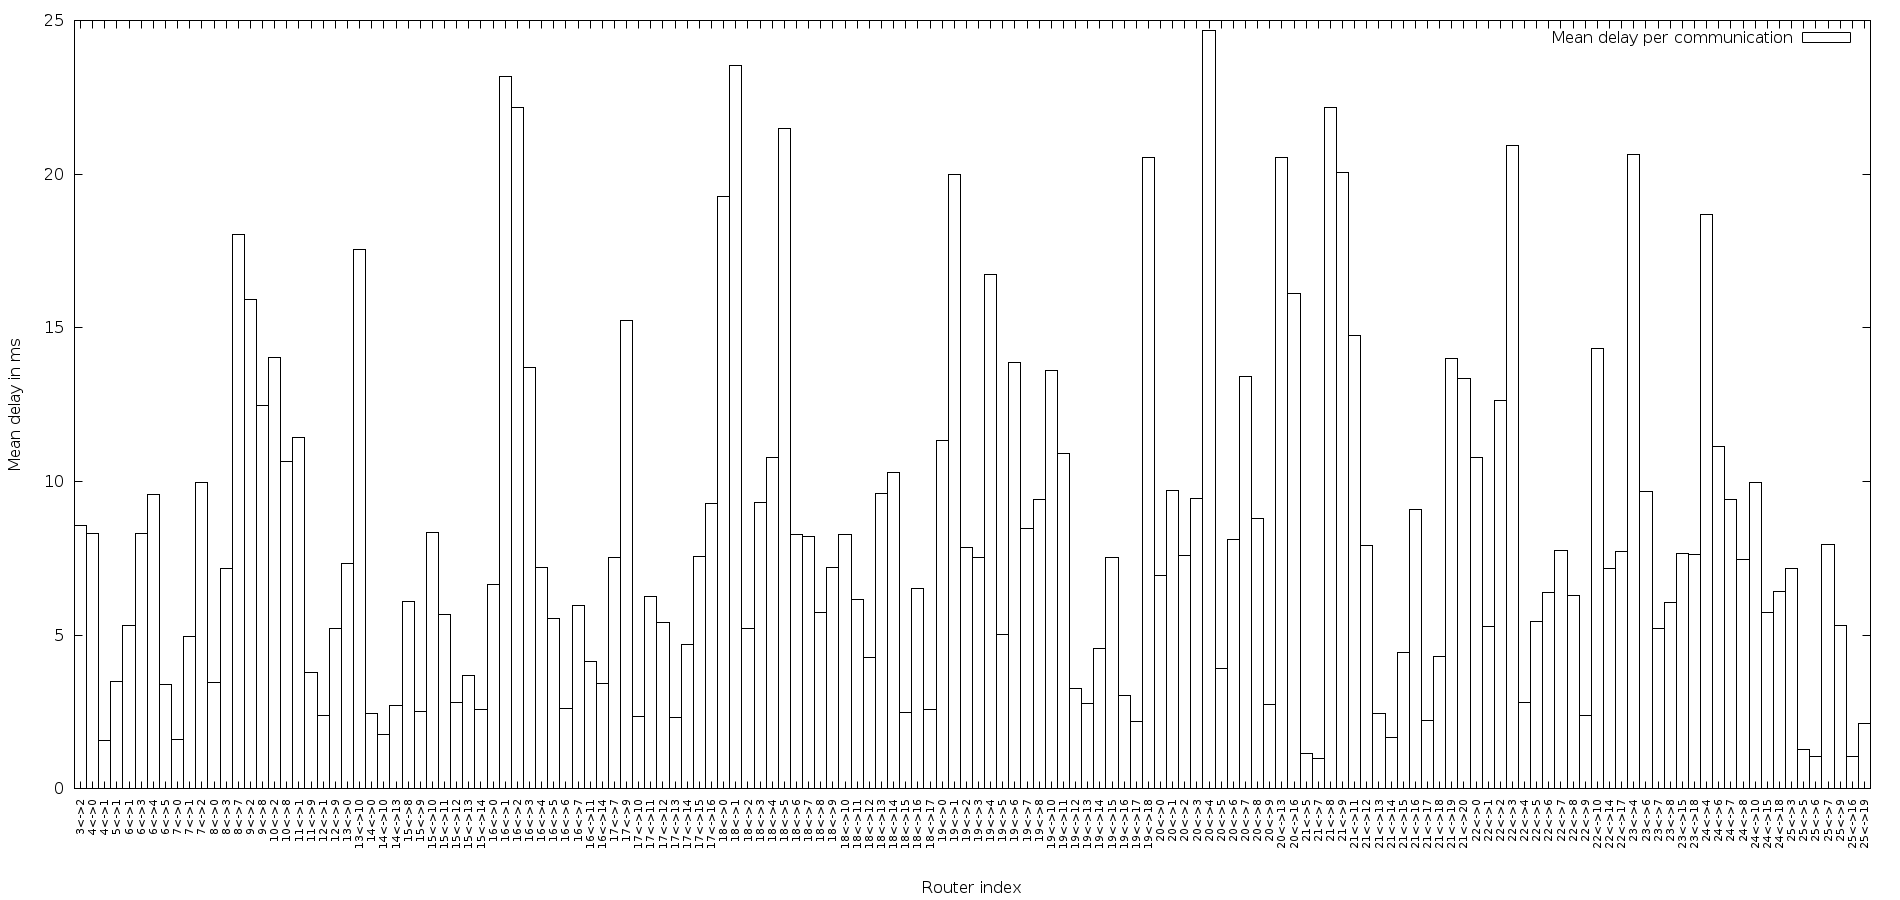
\includegraphics[width=15cm]{png/delay.png}
\end{figure}
%----------------------------------------------------------------------------------------

\newpage % Start the article content on the second page, remove this if you have a longer abstract that goes onto the second page

%----------------------------------------------------------------------------------------
%	I. MANUEL
%----------------------------------------------------------------------------------------

\section{Fonctionnalités implémentées - Manuel d'utilisation}
Le sujet du projet était volontairement assez vague, nous laissant le choix dans les fonctionnalités à implémenter. Il était probablement très dur d'implémenter toutes les fonctionnalités demandées, j'ai donc choisi d'implémenter celles "de base" bien sûr.

Puis j'ai implémenté celles qui m'intéressaient, dans le sens où elles me donneraient une plus grande visibilité sur le réseau ayant produit la trace. Il est en effet impossible de visualiser un réseau de cette ampleur à partir d'une simple trace.
\subsection{Utilisation générale}
	Pour utiliser l'exécutable, il faut forcément l'appeler avec l'option \textit{-f} suivie du nom du fichier à parser, suivies des éventuelles options d'utilisation.
	
	Exemple :
	
	 \centerline{\texttt{\$./trace -f trace2650.txt -p all}}

\subsection{Options}
	Voici les statistiques globales qui sont traitées dans ce projet ainsi qu'un manuel d'utilisation. Toutes les options sont compatibles. Mais ne peuvent-être appelées qu'une fois par exécution. Il n'est donc pas possible de tracer un seul flux et de compter les flux lors d'une seule exécution, par exemple.
	


\subsubsection{\texttt{-f <Nom de fichier>}}
  Indispensable pour préciser le fichier à parser.	

\subsubsection{\texttt{-h}}
Affiche une aide d'utilisation

\subsubsection{\texttt{-F all/N(entier)}}
\begin{itemize}
  \item \textbf{\texttt{all} : }
compte le nombre de flux donnés dans le fichier.\newline \textbf{\texttt{attention} : compter 3 minutes d'exécution}
  \item \textbf{\texttt{N}} (entier) : trace le flux appelé ayant N pour identifiant.
  \item Exemples :\newline\texttt{\$./trace -f trace2650.txt -F all}\newline\texttt{\$./trace -f trace2650.txt -F 2342}
\end{itemize}
\subsubsection{\texttt{-p all/N(entier)}}
\begin{itemize}
\item \textbf{\texttt{all} : }
	réalise un échantillonnage de l'ensemble des paquets injectés dans le réseau toutes les n secondes.
  \item \textbf{\texttt{N}} (entier) : trace le paquet appelé ayant N pour identifiant.
  \item Exemple :\newline\texttt{\$./trace -f trace2650.txt -p 2342}
\end{itemize}

\subsubsection{\texttt{-r all/N(entier)}}
\begin{itemize}
  \item \textbf{\texttt{all}} : affiche le nombre de paquets reçus par chacun des noeuds du réseau.
  \item \textbf{\texttt{N}} (entier) : trace un échantillonnage du nombre de paquets reçus chaque seconde par un routeur. Cette trace est placée dans le dossier \texttt{traces/} et porte le nom de trace\_routeur\textit{N}.tr. On peut ensuite modifier le fichier \texttt{one\_router.gp} pour générer un graphique de cette trace.
  \item Exemples :\newline\texttt{\$./trace -r trace2650.txt -F all}\newline\texttt{\$./trace -r trace2650.txt -F 4}
\end{itemize}
  
\subsubsection{\texttt{-l all}}
\begin{itemize}
  \item \textbf{\texttt{all}} : Affiche un bilan des communication de bout en bout, pour les paires de routeurs ayant communiqué. \newline De plus, créé une trace du nombre de paquets ayant circulé avec succès entre ces routeurs dans \texttt{traces/trace\_delay.tr}
  \item Exemple :\newline\texttt{\$./trace -r trace2650.txt -l all}
\end{itemize}

%----------------------------------------------------------------------------------------
%	II.MEMOIRE ET ALGORITHMIQUE
%----------------------------------------------------------------------------------------

\section{Mémoire et algorithmique}
Le fichier fourni est volumineux puisqu'il pèse plus de 140Mo. De plus, l'utilitaire compatible avec des fichiers bien plus volumineux que celui-ci, pouvant dépasser le Go. 

Aussi chaque choix de conception influe directement sur la vitesse d'éxécution ainsi que par le volume de mémoire vive monopolisé par celui-ci.

Nous n'allons pas détailler l'ensemble du code fourni, mais simplement commenter les points qui ont nécéssité de faire des choix. Commençons par préciser que le fichier n'est parcouru qu'une seule fois et qu'à part pour la fonctionnalité de comptabilisation de tous les flux, le temps d'exécution est inférieur à 5 secondes.



\subsection{Statistiques globales et traçage de flux et paquets}
Il était trivial de comptabiliser les paquets générés et détruits dans l'ensemble du réseau, il suffisait de compter le nombre de code 0 et 4 du fichier.
Pour comptabiliser le nombre de  flux c'était différent puisque la mort et la naissance d'un flux n'étaient jamais clairement marqués. La seule solution était de répertorier tous les identifiants déjà rencontrés. J'ai commis l'erreur de les stocker simplement dans une liste chaînée croissante sans doublon, ce qui rend le temps d'exécution du programme quadratique : en effet, pour chaque ligne du fichier, on parcourt en moyenne toute la liste des flux déjà répertoriés. Il eût été plus judicieux d'utiliser une hashtable. Je n'ai plus reproduit cette erreur pour les autres fonctionnalités.

Concernant le traçage d'un flux ou d'un paquet, il suffisait là aussi de parcourir une seule fois tout le fichier (sauf pour les paquets où l'on pouvait même s'arrêter après la mort du paquet), et de répertorier toutes les informations dans une structure de données adaptée.

\subsection{Statistiques de circulation intra-routeur}
Celle-ci est aussi simple puisqu'il suffit de crééer un tableau de la taille du nombre de routeurs (constante dans \texttt{global.h})et d'incrémenter le nombre de destructions et de passage y ayant lieu. Un tableau de deux entiers par routeur faisait l'affaire.

\subsection{Traçage des délais moyens de communications de bout en bout}
Cette fonctionnalité présentait le plus de défis. Toutes les informations concernant les communications de bout en bout d'un noeud à un autre étaient stockées dans une structure \texttt{links\_charge}. Il est claire que je ne pouvais pas m'y prendre comme je l'avais fait avec les identifiants de flux, puisqu'une liste de listes chaînées aurait immensément accru le temps d'exécution. En effet à chaque réception en un point d'un paquet, il fallait trouver l'évènement correspondant à son émission. Or celui-ci lui étant antérieur, il fallait le stocker. J'ai donc fait deux optimisations :
\begin{itemize}
	\item{Les structures \texttt{links\_charge} contenant les informations pertinentes sur les différents liens, étaient stocké dans un tableau de la taille de $ \frac{  N \times (N-1) }{2} $ } éléments. Une fonction \texttt{get\_hash(i,j)} permettant de renvoyer l'indice de l'élément correspondant à la communication entre i et j. Cette fonction de hash se base sur la linéarisation d'une demi-matrice.
	\item{Il n'est donc pas nécessaire de parcourir tous les \texttt{links\_charge} pour trouver lequel correspond à la ligne du fichier analysé. L'autre optimisation concerne les paquets : une fois qu'on trouve une réception/destruction de paquet, on stocke la durée du voyage puis on supprime le paquet du buffer de paquets dans \texttt{links\_charge}. Ainsi on ne fait que très peu de comparaisons pour trouver où stocker les paquets émis par un noeud.}

\end{itemize}
%----------------------------------------------------------------------------------------
%	II.RÉSULTATS ET EXPLOITATION
%----------------------------------------------------------------------------------------

\newpage
\section{Résultats et exploitation}
Les données collectées concernent trois aspects du réseau :
\begin{itemize}
\item{Ses données globales}
\item{Les données concernant les routeurs (et non les liens)}
\item{Les données concernant les communications de bout en bout}
\end{itemize}

\subsection{Données globales}
\begin{figure}
	\centerfloat
    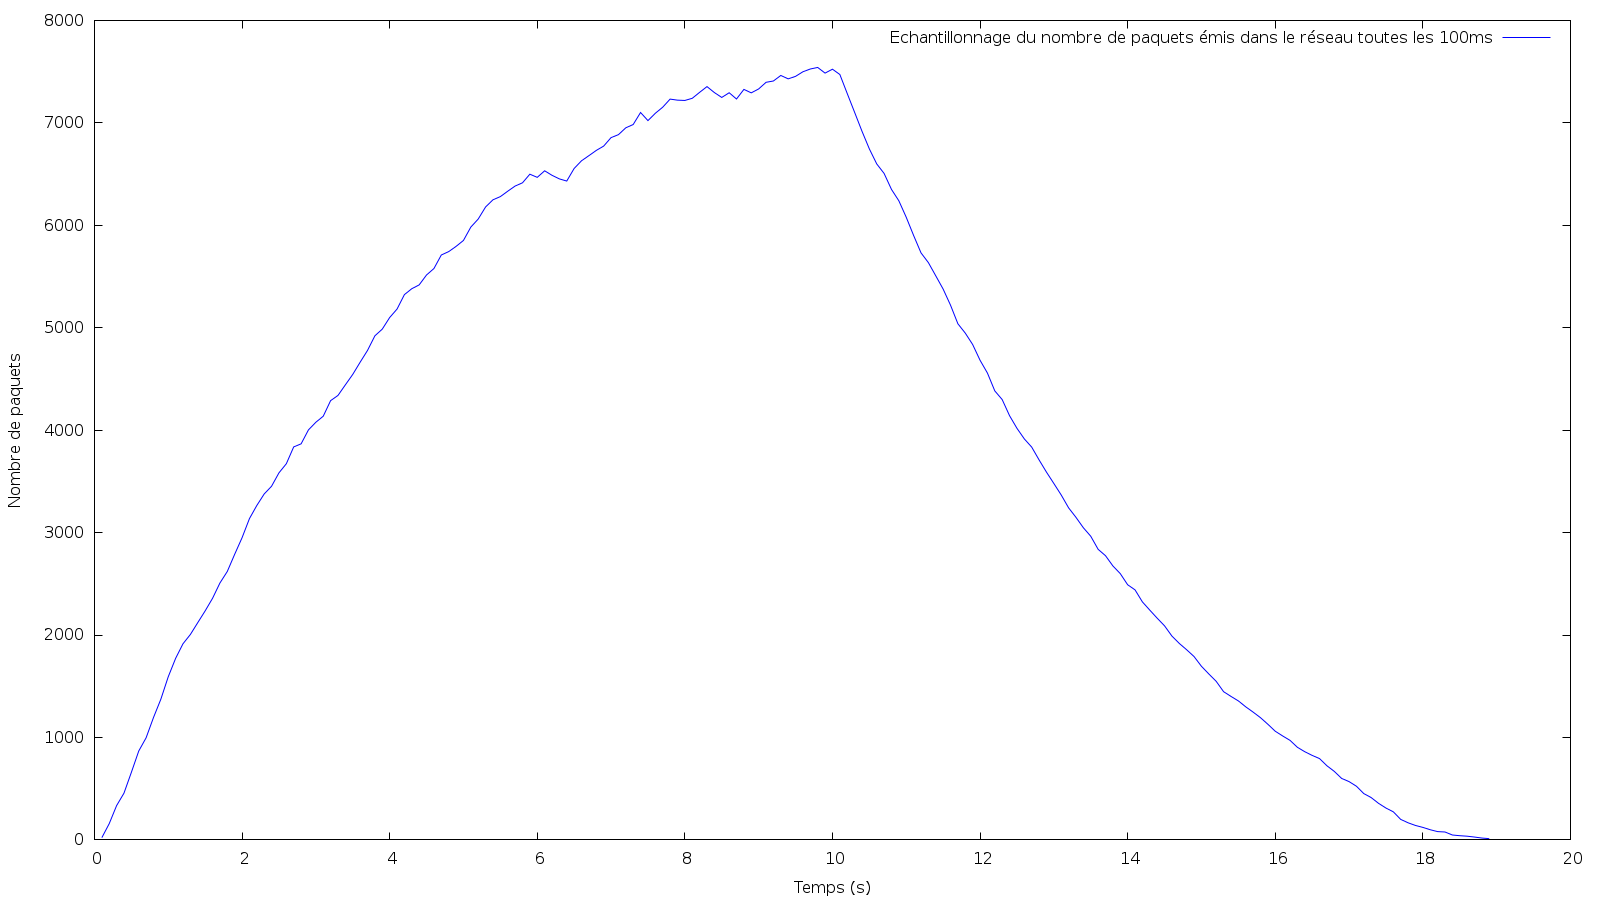
\includegraphics[width=19cm]{png/total_packets.png}
	\caption{Echantillonnage du nombre de paquets émis toutes les 100ms}
   \label{total_packets}
\end{figure}
L'exécutable indique que durant les 20 secondes d'exécution, \textbf{750 979} ont été émis dans le réseau, dont \textbf{35 164} ont été détruits. De plus la figure \ref{total_packets} nous montre la répartition de ces émissions au fil du temps. On constate que l'émission des paquets augmente plutôt linéairement au cours du temps, puis qu'elle s'écroule complètement aux alentours de la $11^{eme} $ seconde, formant une gigantesque dent de scie.

De cela on peut d'ores et déjà déduire une chose : ce réseau n'est pas un réseau uniforme régit par des \textit{Constant Bit Rates} avec des liens et des files de routeurs surdimensionnées. En effet une telle topologie peut signifier plusieurs choses : 
\begin{figure}
	\centerfloat
    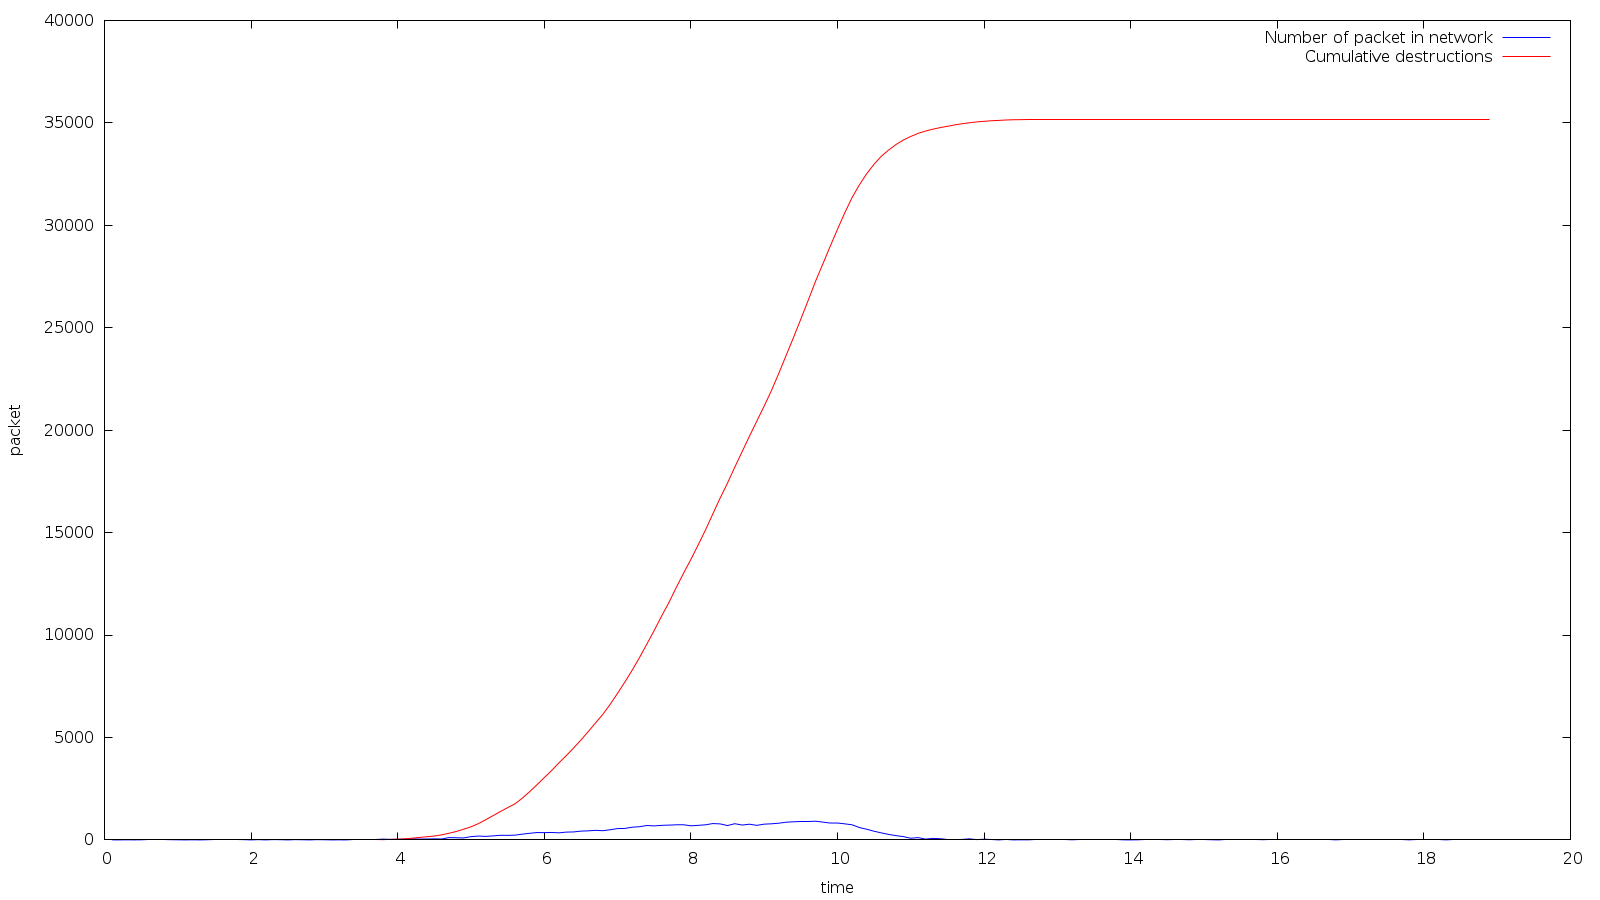
\includegraphics[width=19cm]{png/destr_cumul.png}
	\caption{Echantillonnage du cumul des destructions au cours du temps superposé à la courbe de la Figure \ref{total_packets}}
   \label{total_destroys}
\end{figure}
\begin{itemize}
\item{soit d'une \textbf{congestion} d'un routeur du réseau, qui serait détectée par les émetteurs et qui arrêteraient alors d'émettre.}
\item{soit d'une syncronisation de tous les émetteurs. Peut-être parce qu'ils émettent tous en fonction d'un même algorithme TCP synchronisé par exemple.}
\item{soit d'un trafic généré par une loi "en dent de scie". On en observerait alors simplement une dent dans son intégralité, ce qui serait pertinent comme trace de réseau.}
\end{itemize}

La figure \ref{total_destroys} nous permet néanmoins d'avancer sur la question. En effet on constate qu'à partit de la sixième seconde et jusqu'à la onzième, le nombre de destructions cumulé passe de moins de 5 000 à plus de 35 000 (soit multiplié par sept environ!), puis il stagne.
On peut comprendre que quelque chose se passe sur le réseau. S'il y a destruction, cela signifie qu'un routeur au moins reçoit plus de paquets que ce qu'il pourrait en supporter. La mission consistera donc à déceler le potentiel coupable.



\newpage

\begin{figure}[top]
\centering
\parbox{8cm}{
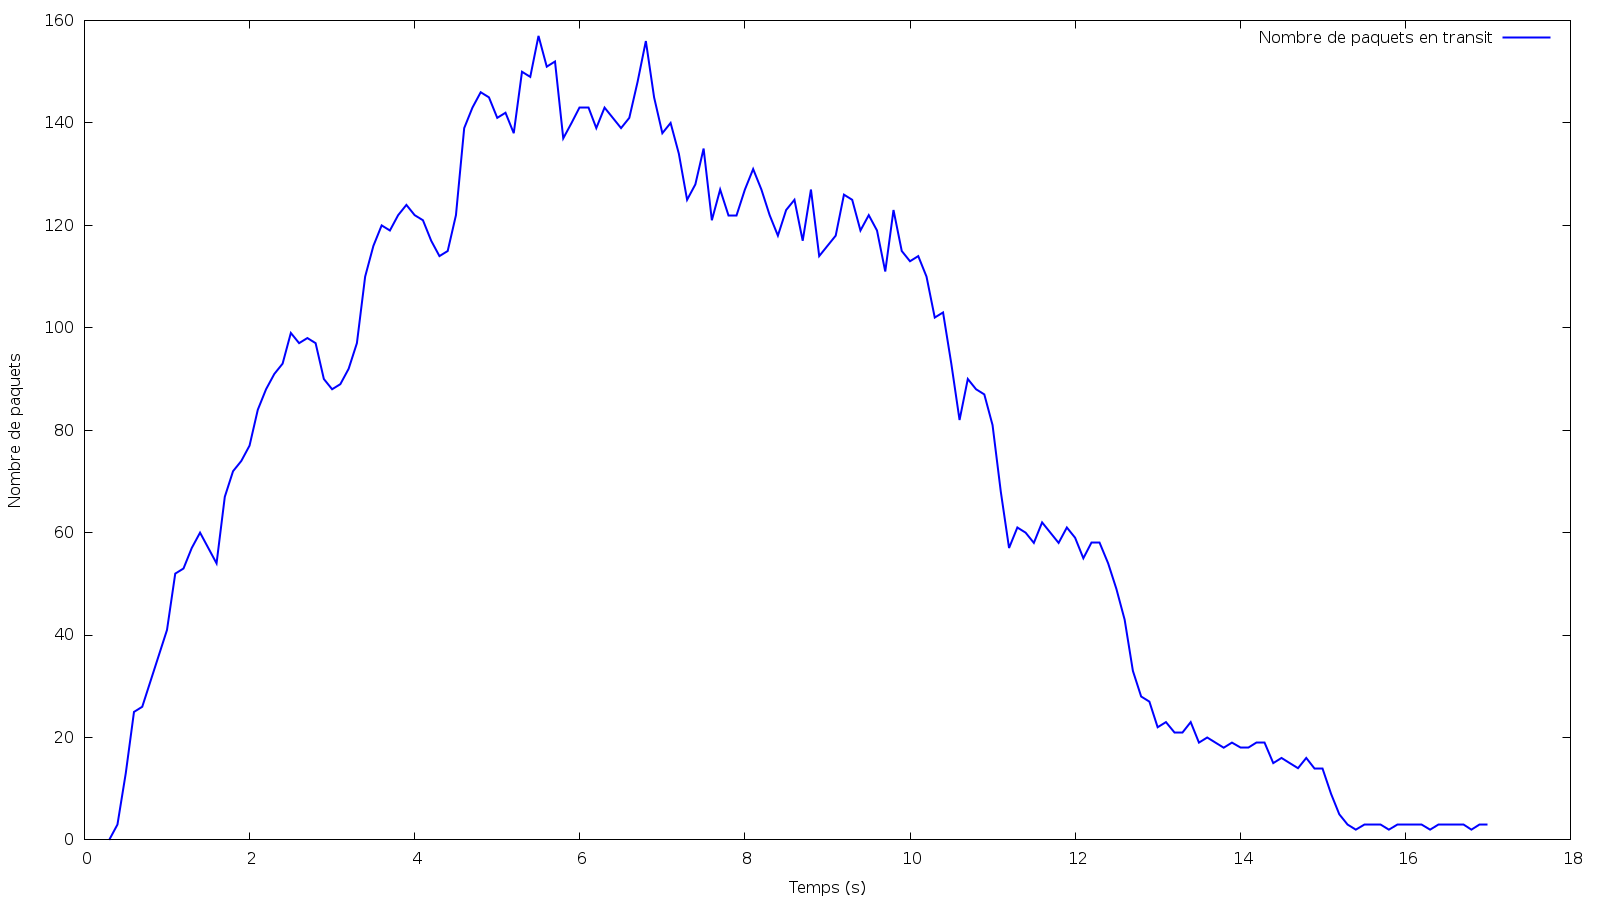
\includegraphics[width=8cm]{png/routers/router3.png}
\caption{Charge des liens également pondérés}
\label{Fair}}
\qquad
\begin{minipage}{8cm}
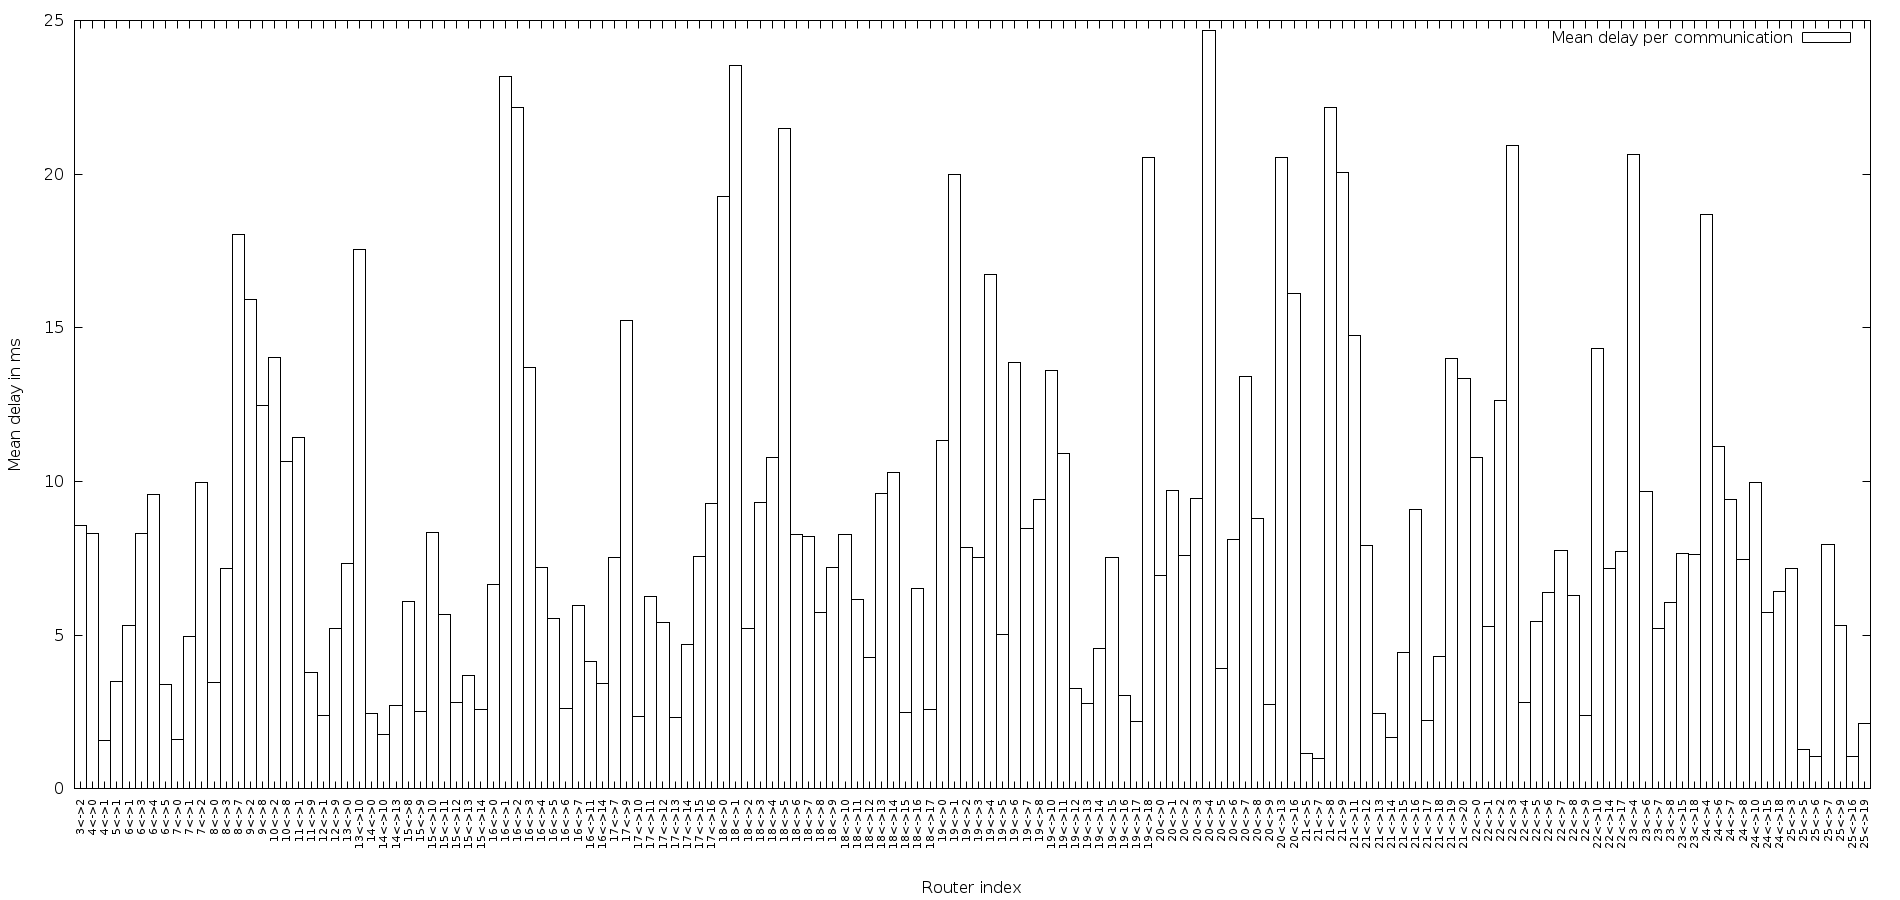
\includegraphics[width=8cm]{png/delay.png}
\caption{Charge des liens avec le lien 1-2 plus couteux}
\label{Unfair}
\end{minipage}
\begin{minipage}{8cm}
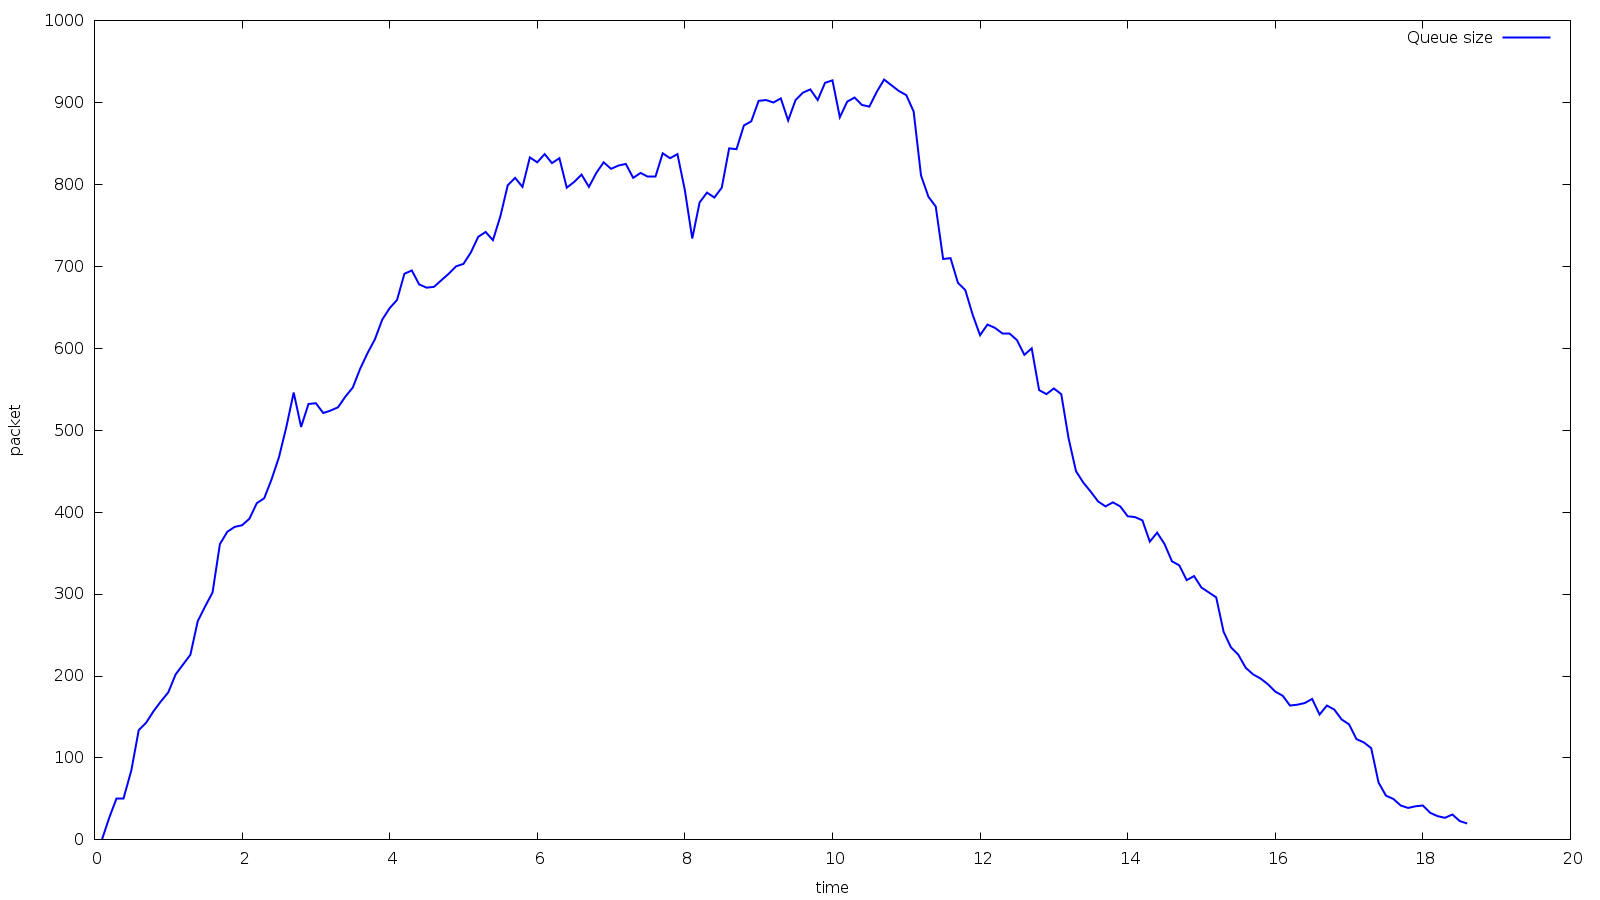
\includegraphics[width=8cm]{png/routers/router20.png}
\caption{Routage plus équitable}
\label{Eq}
\end{minipage}
\end{figure}



\end{document}
